%%%%%%%%%%%%%%%%%%%%%%%%%%%%%%%%%%%%%%%%%
% Short Sectioned Assignment
% LaTeX Template
% Version 1.0 (5/5/12)
%
% This template has been downloaded from:
% http://www.LaTeXTemplates.com
%
% Original author:
% Frits Wenneker (http://www.howtotex.com)
%
% License:
% CC BY-NC-SA 3.0 (http://creativecommons.org/licenses/by-nc-sa/3.0/)
%
%%%%%%%%%%%%%%%%%%%%%%%%%%%%%%%%%%%%%%%%%

%----------------------------------------------------------------------------------------
%   PACKAGES AND OTHER DOCUMENT CONFIGURATIONS
%----------------------------------------------------------------------------------------

\documentclass[paper=letter, fontsize=11pt]{scrartcl} % A4 paper and 11pt font size
\synctex=1
\usepackage[T1]{fontenc} % Use 8-bit encoding that has 256 glyphs
\usepackage{fourier} % Use the Adobe Utopia font for the document - comment this line to return to the LaTeX default
\usepackage[english]{babel} % English language/hyphenation
\usepackage{amsmath,amsfonts,amsthm} % Math packages
%\usepackage[nolists, nomarkers]{endfloat}
\usepackage{hyperref}
\usepackage{bm}
\usepackage{graphicx}
\usepackage[section]{placeins}
\usepackage{sectsty} % Allows customizing section commands
\allsectionsfont{\normalfont\scshape} % Make all sections centered, the default font and small caps

\usepackage{fancyhdr} % Custom headers and footers
\pagestyle{fancyplain} % Makes all pages in the document conform to the custom headers and footers
\fancyhead{} % No page header - if you want one, create it in the same way as the footers below
\fancyfoot[L]{} % Empty left footer
\fancyfoot[C]{} % Empty center footer
\fancyfoot[R]{\thepage} % Page numbering for right footer
\renewcommand{\headrulewidth}{0pt} % Remove header underlines
\renewcommand{\footrulewidth}{0pt} % Remove footer underlines
\setlength{\headheight}{13.6pt} % Customize the height of the header

\numberwithin{equation}{section} % Number equations within sections (i.e. 1.1, 1.2, 2.1, 2.2 instead of 1, 2, 3, 4)
\numberwithin{figure}{section} % Number figures within sections (i.e. 1.1, 1.2, 2.1, 2.2 instead of 1, 2, 3, 4)
\numberwithin{table}{section} % Number tables within sections (i.e. 1.1, 1.2, 2.1, 2.2 instead of 1, 2, 3, 4)

\setlength\parindent{0pt} % Removes all indentation from paragraphs -
                          % comment this line for an assignment with
                          % lots of text
\setlength\parskip{12pt}

%----------------------------------------------------------------------------------------
%   TITLE SECTION
%----------------------------------------------------------------------------------------

\newcommand{\horrule}[1]{\rule{\linewidth}{#1}} % Create horizontal rule command with 1 argument of height

\title{ 
\normalfont \normalsize 
\textsc{Exoplanet Patchy Cloud Project} \\ [25pt] % Your university, school and/or department name(s)
\horrule{0.5pt} \\[0.4cm] % Thin top horizontal rule
\huge Data Preparation\\ % The assignment title
\horrule{2pt} \\[0.5cm] % Thick bottom horizontal rule
}

\author{Yifan Zhou} % Your name

\date{\normalsize\today} % Today's date or a custom date

\begin{document}

\maketitle % Print the title
\section{Summary}
\begin{enumerate}
\item Cross correlation has the best performance for locating the
  centroids of star images.
\item Bicubic interpolation generates smaller RMS fluctuation
  comparing to \texttt{FSHIFT.pro} when shift images, but does not
  strictly obey flux conservation. \texttt{FSHIFT.pro} strictly keeps
  the conservation of flux. Bicubic interpolation causes artifacts
  around the star images.
\end{enumerate}

\section{Centroid of Primary Star}
4 methods to locate the centroid of the primary objects were tested
for all 78 cosmic ray removed images of ABPIC-B. I compared the 4 sets
of results in order to determine the best method to find star image
centroid in this situation where the image is slightly saturated.\par

\subsection{Method Introduction}

\begin{enumerate}
\item \texttt{CNTRD.PRO}\\
  IDL routine \texttt{CNTRO.PRO} locates the position where the X
  and Y derivatives go to zero. The search area of \texttt{CNTRO.PRO}
  can be adjusted with parameter \texttt{EXTENDBOX}.\par
\item \texttt{GCNTRD.PRO}\\
  IDL routine \texttt{GCNTRD.PRO} fits the star image with a 2D-Gaussian
  function to search for centroid. The search area cannot be defined
  in this routine. \texttt{GCNTRD.pro} is likely to fail when the
  initial guess of centroid coordinates are far away from the true
  values. This is inconvenient for pipeline scenario, where images
  of different dithering positions are assigned with same initial
  values for fitting. In practice, I ran \texttt{CNTRD.PRO} before
  \texttt{GCNTRD.PRO} to provide initial values for Gaussian fitting.\par
\item Cross Correlation\\
  Calculate the cross correlation value to align images. The images
  taken with different rolling angle were treat separately. Images
  taken in 1st, 3th, and 5th orbits were calculated cross correlation
  with the first image in 1st orbit and images taken in 2nd, 4th, and
  6th orbits with first image in 2nd orbit.\par
 \item World Coordinate System(WCS)\\
   Use WCS to align every image. The treatment with different rolling
   angles is the same as cross correlation method. Centroids were
   calculated with IDL routine \texttt{XYXY.pro}.\par
\end{enumerate}

\subsection{Result Comparison}
Figure \ref{fig:x_off} and \ref{fig:y_off} demonstrates the
distributions of centroid offsets of \texttt{GCNTRD.pro}, cross
correlation, and WCS relative to the \texttt{CNTRD.pro} method in $x$
and $y$ direction. \par

According to the two plots, most of results calculated with all four
methods are constrained within $\pm 0.2$ pixels. Both in $x$ and $y$
directions, the histograms of \texttt{GCNTRD.pro} offsets have a
fairly strange shape, while the distributions of cross correlation and
WCS methods' offsets show a Gaussian like shape. In $x$-direction, the
distributions of cross correlation and WCS have similar behavior that
the centers of two histograms both have $\sim -0.1$ pixels offset. In
$y$ direction, histogram of cross correlation demonstrates that the
results for cross correlation and \texttt{CNTRD.pro} are well
agreed. The histogram of WCS is skewed and has a $\sim -0.1$ pixels
offset.\par

To sum, \texttt{GCNTRD.pro} method has the worst performance. In
$x$-direction, the results for cross correlation and WCS agrees well
and in $y$-direction the results for cross correlation and
\texttt{CNTRD.pro} agrees well. Thus cross correlation method performs
best.\par

\begin{figure}
  \centering
  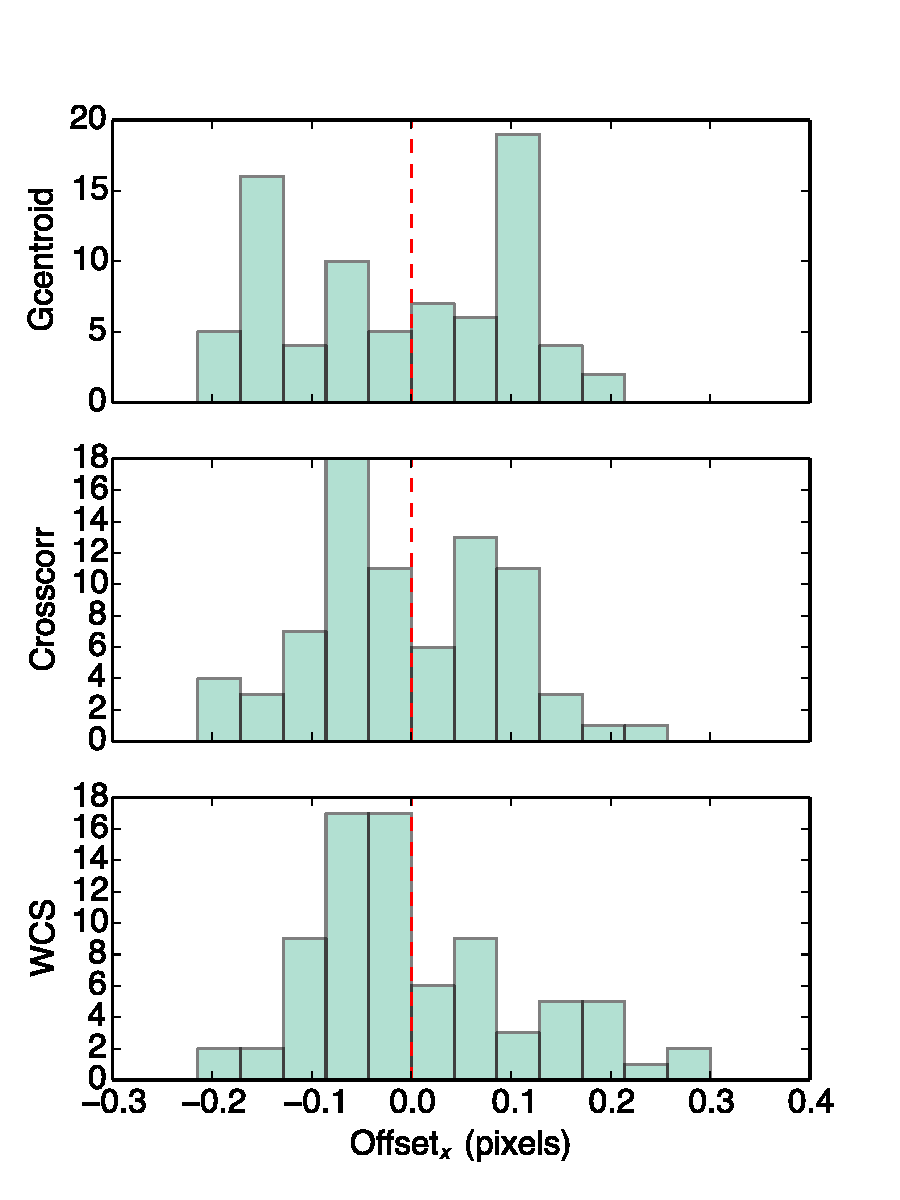
\includegraphics[width=\textwidth]{x_off}
  \caption{$x$-direction offset histogram}
  \label{fig:x_off}
\end{figure}
\begin{figure}
  \centering
  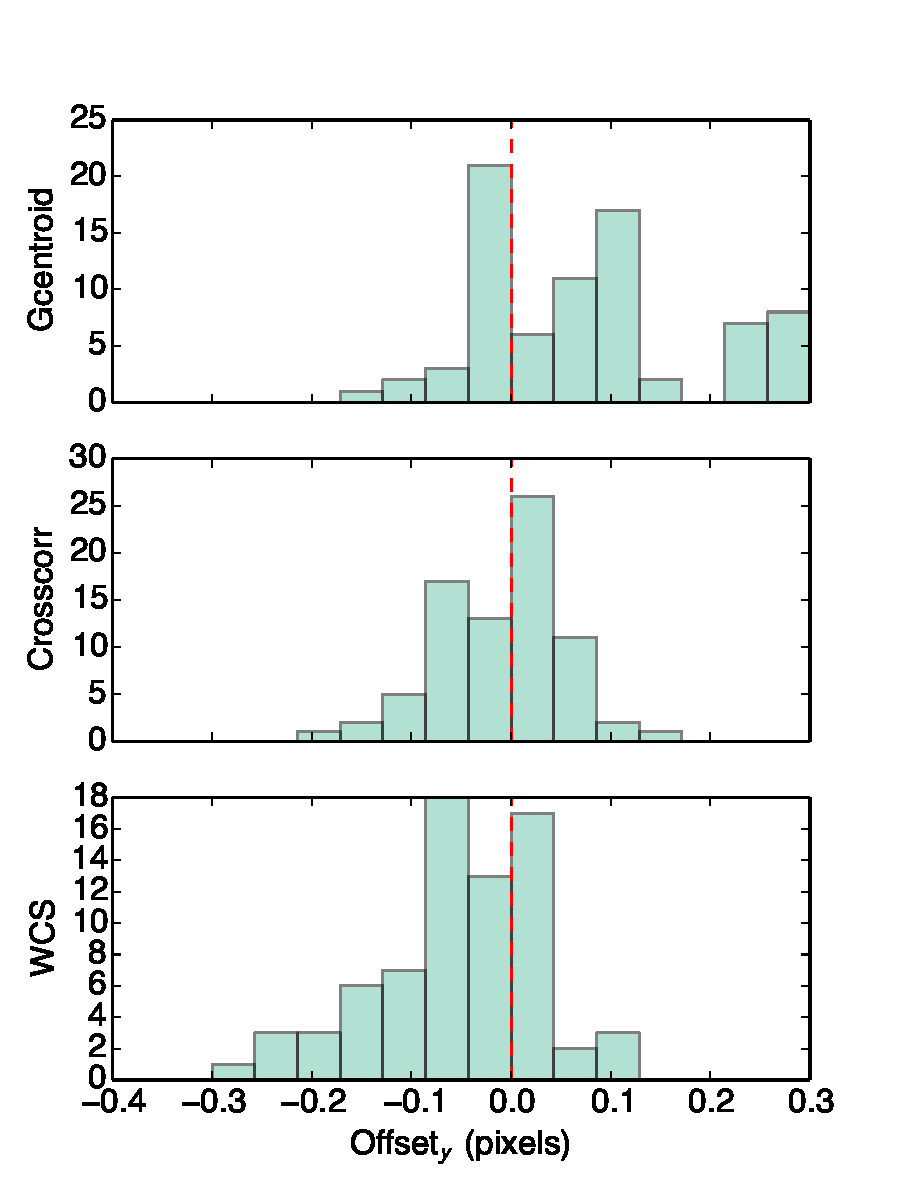
\includegraphics[width=\textwidth]{y_off}
  \caption{$y$-direction offset histogram}
  \label{fig:y_off}
\end{figure}

\section{Image shift and interpolation algorithm}

I tested two image shift methods that uses two different interpolation
algorithms. The two algorithms are bicubic interpolation and bilinear
interpolation(used by  IDL routine \texttt{FSHIFT.pro}).\par

To evalueate the two shift methods, the image is shifted in a random direction
with a specific length and then shifted back. Both the root mean
square and mean flux change between the original image and the
modified image  will be calculated as following:
\begin{align}
  &\Delta_{\mathrm{rms}} = \frac{\sqrt{(\mathrm{img}_{0} -
      \mathrm{img_{shifted}})^{2}}}{N_{\mathrm{pixels}}}\\
  &\bar{\Delta} = \frac{\mathrm{img}_{0} - \mathrm{img_{shifted}}}{N_{\mathrm{pixels}}}
\end{align}

The results are demonstrated with figure \ref{fig:shifted}.
\begin{figure}[h]
  \centering
  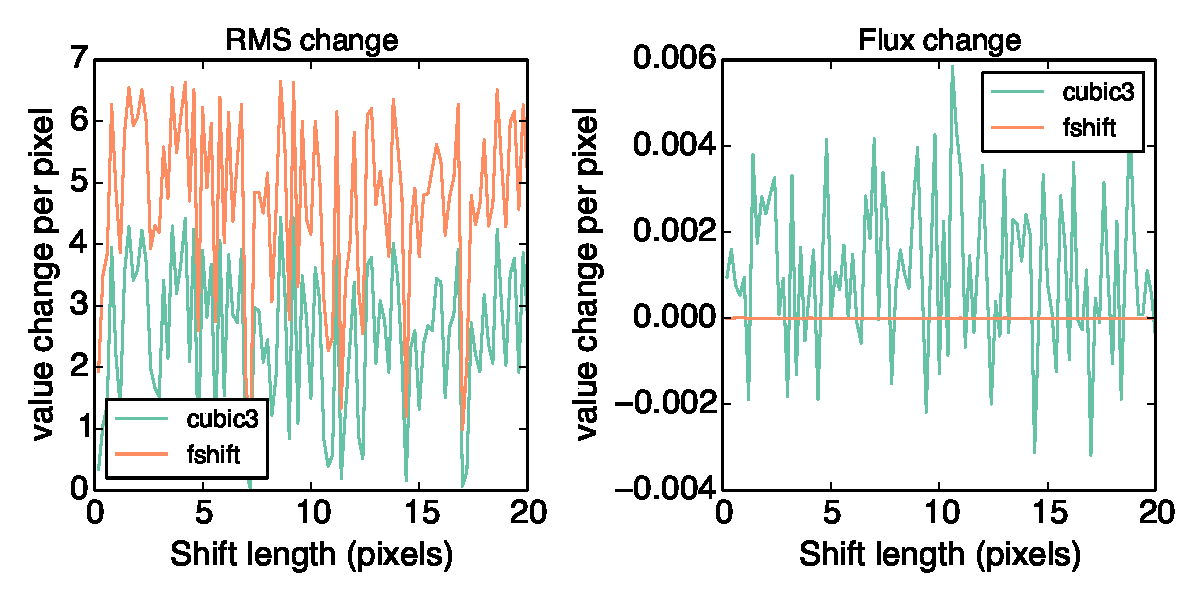
\includegraphics[width=\textwidth]{test_shift}
  \caption{Root mean square and mean flux change betwenn the original image and the modified image as a function of shift length.}
  \label{fig:shifted}
\end{figure}
\begin{enumerate}
\item bicubic interpolation comes up with a smaller RMS change, thus
  the error generated by image shift will be smaller with a bicubic interpolation.
\item \texttt{FSHIFT.pro} strictly keeps flux conserved, while bicubic
  interpolation ends up with a $\sim \pm 0.003$ per pixel change in flux.
\item bicubic interpolation will generate ringing artifacts(figure \ref{fig:ringing})
\end{enumerate}
\begin{figure}[h]
  \centering
  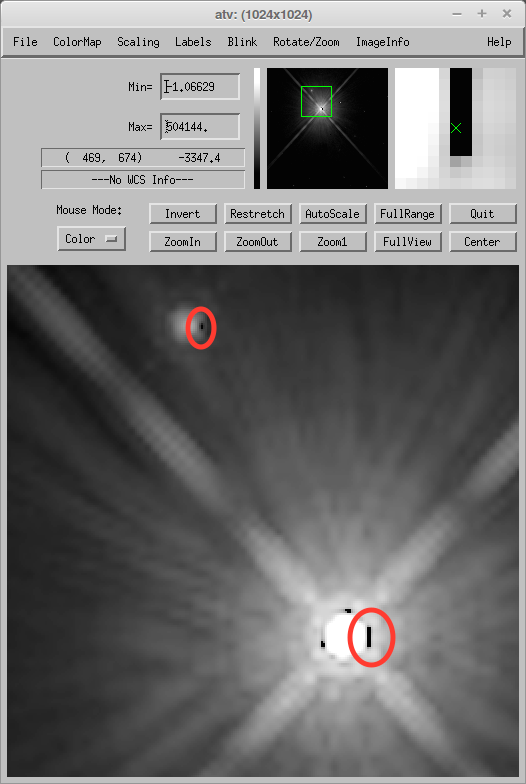
\includegraphics[width=0.6\textwidth]{interpolated}
  \caption{Ringing artifacts generated by bicubic interpolation.}
  \label{fig:ringing}
\end{figure}
\end{document}
%%% Local Variables:
%%% mode: latex
%%% TeX-master: t
%%% End:
